% --- IMPORTS ---
\documentclass[leqno]{article}
\usepackage{graphicx}
\usepackage{dsfont}
\usepackage{mathtools}
\usepackage{amssymb}
\usepackage{amsmath}
\usepackage{amsthm}
\usepackage{float}
\usepackage{ragged2e}
\usepackage{tensor}
\usepackage{fancyhdr}
\usepackage{empheq}
\usepackage[most]{tcolorbox}
\usepackage{enumitem}
\usepackage{dirtytalk}
\usepackage{marginnote}
\usepackage{microtype}
\usepackage[
  a4paper,
  left=0.8in,
  right=1in,
  top=1in,
  bottom=0.5in,
  headheight=14pt,
  headsep=0.4in
]{geometry}
\setlength{\parindent}{0cm}
% --- TikZ Packages ---
\usepackage{pgfplots}
\pgfplotsset{compat=1.18}
\usepgfplotslibrary{fillbetween, polar}
\usetikzlibrary{calc, positioning}
\usetikzlibrary{angles, quotes}
\usetikzlibrary{arrows.meta}
\usetikzlibrary{decorations.pathreplacing, decorations.markings}
\usetikzlibrary{patterns}
\usetikzlibrary{intersections}
% --- URL Packages ---
\usepackage[colorlinks=true,linkcolor=red,citecolor=magenta,urlcolor=black]{hyperref}%
\urlstyle{same}
% --- END OF IMPORTS ---

% --- CUSTOM COMMANDS ---
\RenewDocumentCommand{\marks}{o m}{%
  \IfValueTF{#1}%
    {\marginnote{\raggedright\textbf{[#2]}}[#1]}%
    {\marginnote{\raggedright\textbf{[#2]}}}%
}
\newcommand{\vspacerule}[2]{%
  \par\vspace*{#1}%
  \noindent\hrulefill\par
  \vspace*{#2}%
}
\definecolor{scarlet}{RGB}{205, 40, 75}
\newcommand{\questionitem}{%
  \item\phantomsection
  \addcontentsline{toc}{section}{Question \number\value{enumi}}%
}
\renewcommand{\contentsname}{Questions}
% --- END OF CUSTOM COMMANDS ---

% --- HEADER CONFIG ---
\pagestyle{fancy}
\fancyhead{}
\fancyfoot{}
\renewcommand{\headrulewidth}{0.9pt}
\lhead{Tangents to Polar Curves}
\chead{}
\rhead{\href{https://danieljsmith.org}{danieljsmith.org}}
% --- END OF HEADER CONFIG ---

\begin{document}
\vspace*{20pt}
\tableofcontents
\newpage
\begin{enumerate}[
  label=\textbf{\arabic*.},
  leftmargin=*,
  topsep=0pt,
  partopsep=0pt,
  parsep=0pt
]


% ---- Question 1 ----
\questionitem

\begin{figure}[H]
    \centering
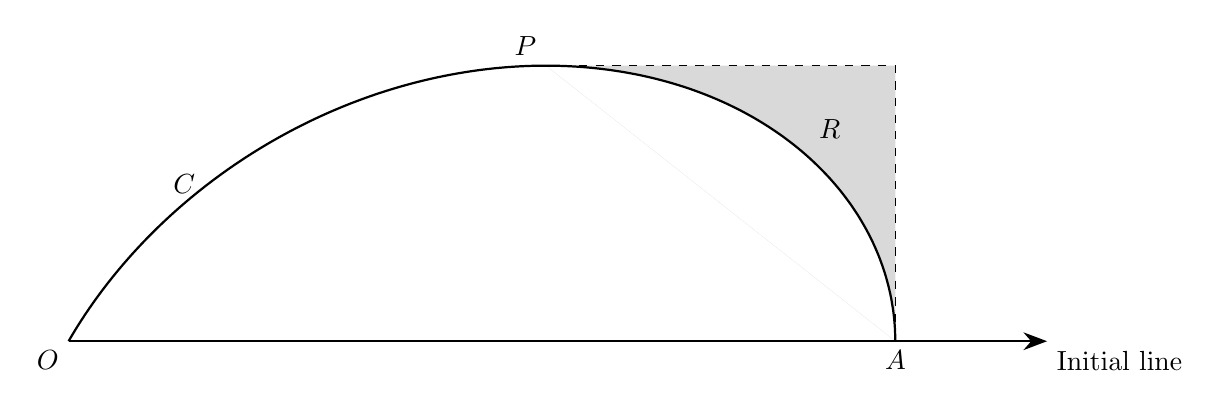
\begin{tikzpicture}[scale=3.5]
\def\thP{30}
\def\thMax{60}
\def\thC{50}
\pgfmathsetmacro{\rP}{1 + 2*cos(2*\thP)}
\pgfmathsetmacro{\xP}{\rP*cos(\thP)}
\pgfmathsetmacro{\yP}{\rP*sin(\thP)}
\coordinate (O) at (0,0);
\coordinate (A) at (3,0);
\coordinate (P) at (\xP,\yP);
\coordinate (T) at (3,\yP);
\coordinate (I) at (3.55,0);
\coordinate (CL) at ({(1 + 2*cos(2*\thC))*cos(\thC)},{(1 + 2*cos(2*\thC))*sin(\thC)});
\coordinate (Rlabel) at ($(A)!0.52!(P)+(0.42,0.25)$);

\fill[gray!30] (P) -- (T) -- (A)
  plot[smooth, samples=120, domain=0:\thP]
    ({(1 + 2*cos(2*\x))*cos(\x)},{(1 + 2*cos(2*\x))*sin(\x)})
  -- cycle;

\draw[-{Stealth[length=3mm]}, thick] (O) -- (I);
\draw[thick] plot[smooth, samples=200, domain=0:\thMax]
  ({(1 + 2*cos(2*\x))*cos(\x)},{(1 + 2*cos(2*\x))*sin(\x)});
\draw[dashed] (P) -- (T) -- (A);

\node[below left] at (O) {$O$};
\node[below] at (A) {$A$};
\node[above left] at (P) {$P$};
\node[above] at (CL) {$C$};
\node at (Rlabel) {$R$};
\node[below right] at (I) {Initial line};
\end{tikzpicture}
\end{figure}


The curve $C$ shown in the figure above has polar equation
\[
r = 1 + 2\cos 2\theta, \qquad 0 \leq \theta \leq \frac{\pi}{3}
\]
\\
At the point $P$ on $C$, the tangent to $C$ is parallel to the initial line. \\

\begin{enumerate}[label=\textbf{(\alph*)}]
  \item Show that $P$ has polar coordinates $\left(2, \dfrac{\pi}{6}\right)$. \marks{4} \\
\end{enumerate}
The point $A$ on $C$ has polar coordinates $(3, 0)$. \\

The finite region $R$, shown shaded in the figure above, is bounded by the arc $AP$ of $C$, the tangent to $C$ at $P$ and the line through $A$ parallel to $\theta = \frac{\pi}{2}$. \\
\begin{enumerate}[label=\textbf{(\alph*)}, resume]
  \item Find the exact area of $R$. \marks{9} \\
\end{enumerate}
\newpage
% ---- Question 2 ----
\questionitem

The curve $C$ has polar equation
\[
r = 2\sin 3\theta, \qquad 0 \leq \theta \leq \frac{\pi}{3}
\]
\\
At the non-pole point $P$ on $C$, the tangent to $C$ is parallel to the initial line. \\

Given that $O$ is the pole, find the exact length of the line $OP$. \marks{7}

\newpage


% ---- Question 3 ----
\questionitem

\begin{figure}[H]
    \centering
\begin{tikzpicture}[scale=1.5]
\def\rA{2}
\def\k{0.60}
\def\thP{0.82}
\pgfmathsetmacro{\rP}{\rA*exp(\k*\thP)}
\pgfmathsetmacro{\xP}{\rP*cos(deg(\thP))}
\pgfmathsetmacro{\yP}{\rP*sin(deg(\thP))}
\pgfmathsetmacro{\dx}{\rP*(\k*cos(deg(\thP)) - sin(deg(\thP)))}
\pgfmathsetmacro{\dy}{\rP*(\k*sin(deg(\thP)) + cos(deg(\thP)))}
\pgfmathsetmacro{\tT}{-\yP/\dy}
\pgfmathsetmacro{\xT}{\xP + \tT*\dx}
\pgfmathsetmacro{\tQ}{0.75}
\pgfmathsetmacro{\xQ}{\xP + \tQ*\dx}
\pgfmathsetmacro{\yQ}{\yP + \tQ*\dy}
\pgfmathsetmacro{\xEnd}{\xT + 0.55}
\pgfmathsetmacro{\thC}{1.3}
\pgfmathsetmacro{\rC}{\rA*exp(\k*\thC)}
\pgfmathsetmacro{\xC}{\rC*cos(deg(\thC))}
\pgfmathsetmacro{\yC}{\rC*sin(deg(\thC))}

\coordinate (O) at (0,0);
\coordinate (I) at (1,0);
\coordinate (A) at (\rA,0);
\coordinate (P) at (\xP,\yP);
\coordinate (T) at (\xT,0);
\coordinate (Q) at (\xQ,\yQ);
\coordinate (CLabel) at (\xC,\yC);

\draw[thick] (O) -- (\xEnd,0);
\draw[dashed] (O) -- (P);
\draw[thick] (Q) -- (T);
\draw[thick, black] plot[smooth, samples=160, domain=0:1.30, variable=\t]
  ({\rA*exp(\k*\t)*cos(deg(\t))},{\rA*exp(\k*\t)*sin(deg(\t))});

\pic["$\theta$", draw, angle radius=5mm, angle eccentricity=1.35]
  {angle=I--O--P};

\node[below left] at (O) {$O$};
\node[below] at (A) {$A$};
\node[right] at (P) {$P$};
\node[below] at (T) {$T$};
\node[above] at (Q) {$Q$};
\node[below left] at (CLabel) {$C$};
\draw[-{Stealth[length=3mm]}, thick] (O) -- (4.5, 0)
  node[pos=0.95, below] {Initial line};
\end{tikzpicture}
\end{figure}


The diagram shows part of a spiral $C$. \\

The point $P$ has polar coordinates $(r, \theta)$, where $0 \leq \theta \leq \frac{\pi}{2}$. \\

The tangent at $P$ is the line $TPQ$. The point $A$ lies on $C$ and on the initial line, with $OA = 2$. \\

Let $\psi$ be the angle that $TPQ$ makes with the initial line. \\

\begin{enumerate}[label=\textbf{(\alph*)}]
  \item By expressing the Cartesian coordinates of $P$ in terms of $r$ and $\theta$, show that
  \[
  \tan \psi = \frac{\frac{\mathrm{d}r}{\mathrm{d}\theta}\sin\theta + r\cos\theta}{\frac{\mathrm{d}r}{\mathrm{d}\theta}\cos\theta - r\sin\theta}
  \]
  \marks[-30pt]{4}
  \item The spiral is equiangular: at every point $P$, the acute angle between $OP$ and $TPQ$ is a constant $\alpha$, where $0 < \alpha < \frac{\pi}{2}$. \\

  Use the result of part (a) to show that the polar equation of $C$ is
  \[
  r = 2e^{(\cot \alpha)\theta}
  \]
  \marks[-20pt]{7}
\end{enumerate}


\newpage

% ---- Question 4 ----
\questionitem

\begin{figure}[H]
    \centering
\begin{tikzpicture}[scale=1.5]
\def\axislen{5.2}
\def\labang{60}
\draw[-{Stealth[length=3mm]}, thick] (0,0) -- (\axislen,0) node[pos=0.95, below] {Initial line};
\draw[thick, black]
  plot[smooth, samples=300, domain=-180:180]
    ({2*(1+cos(\x))*cos(\x)},{2*(1+cos(\x))*sin(\x)});
\coordinate (L) at ({2*(1+cos(\labang))*cos(\labang)},{2*(1+cos(\labang))*sin(\labang)});
\node[above right] at (L) {$C_1$};
\node[below] at (0,0) {$O$};
\end{tikzpicture}
\end{figure}


The diagram shows the sketch of a curve $C_1$. \\

The polar equation of the curve $C_1$ is
\[
r = 2(1 + \cos \theta), \qquad -\pi \leq \theta \leq \pi
\]
\begin{enumerate}[label=\textbf{(\alph*)}]
  \item Find the area of the region bounded by the curve $C_1$. \marks{5} \\
  \item The curve $C_2$ whose polar equation is
  \[
  r = \sin \theta, \qquad 0 \leq \theta \leq \pi
  \]
  intersects the curve $C_1$ at the pole $O$ and at the point $A$. The straight line drawn through $A$ perpendicular to the initial line intersects the part of $C_1$ above the initial line again at the point $B$. \\
  \begin{enumerate}[label=(\roman*)]
    \item Find the polar coordinates of $A$. \marks{4}
    \item Show that the length of $OB$ is $\dfrac{6}{5}$. \marks{6}
    \item Find the length of $AB$, giving your answer to three significant figures. \marks{3}
  \end{enumerate}
\end{enumerate}

\newpage

% ---- Question 5 ----
\questionitem

The curve $C$ has polar equation
\[
r = 3\sin 2\theta, \qquad 0 \leq \theta \leq \frac{\pi}{2}
\]
\\
At the non-pole point $P$ on $C$, the tangent to $C$ is perpendicular to the initial line. \\

Given that $O$ is the pole, find the exact length of the line $OP$. \marks{7}

\newpage

% ---- Question 6 ----
\questionitem

\begin{figure}[H]
    \centering
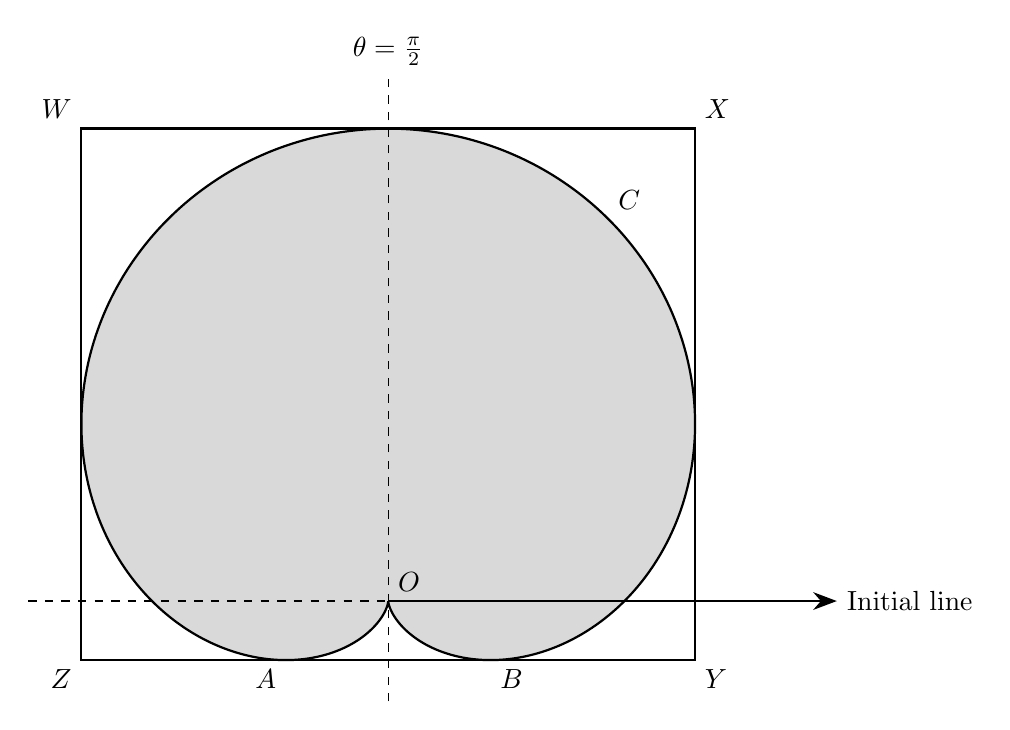
\begin{tikzpicture}[scale=1.5]
\def\a{2}
\pgfmathsetmacro{\xleft}{-3*sqrt(3)*\a/4}
\pgfmathsetmacro{\xright}{3*sqrt(3)*\a/4}
\pgfmathsetmacro{\ytop}{2*\a}
\pgfmathsetmacro{\ybottom}{-\a/4}
\pgfmathsetmacro{\xab}{sqrt(3)*\a/4}

\coordinate (O) at (0,0);
\coordinate (W) at (\xleft,\ytop);
\coordinate (X) at (\xright,\ytop);
\coordinate (Y) at (\xright,\ybottom);
\coordinate (Z) at (\xleft,\ybottom);
\coordinate (A) at (-\xab,\ybottom);
\coordinate (B) at (\xab,\ybottom);
\coordinate (Clbl) at ({\a*(1+sin(60))*cos(60)},{\a*(1+sin(60))*sin(60)});

\fill[gray!30]
  plot[smooth, samples=300, domain=-1.570796:4.712389]
    ({\a*(1+sin(deg(\x)))*cos(deg(\x))},{\a*(1+sin(deg(\x)))*sin(deg(\x))})
  -- cycle;

\draw[thick] (W) -- (X) -- (Y) -- (Z) -- cycle;
\draw[dashed] (\xleft-0.45,0) -- (O);
\draw[dashed] (0,\ybottom-0.35) -- (0,\ytop+0.45);
\draw[-{Stealth[length=3mm]}, thick] (O) -- (\xright+1.2,0) node[right] {Initial line};

\draw[thick]
  plot[smooth, samples=300, domain=-1.570796:4.712389]
    ({\a*(1+sin(deg(\x)))*cos(deg(\x))},{\a*(1+sin(deg(\x)))*sin(deg(\x))});

\node[above left] at (W) {$W$};
\node[above right] at (X) {$X$};
\node[below right] at (Y) {$Y$};
\node[below left] at (Z) {$Z$};
\node[below left] at (A) {$A$};
\node[below right] at (B) {$B$};
\node[above right] at (O) {$O$};
\node[above] at (0,\ytop+0.45) {$\theta=\frac{\pi}{2}$};
\node[above right] at (Clbl) {$C$};
\end{tikzpicture}
\end{figure}


The figure shows a sketch of the cardioid $C$ with equation
\[
r = a(1 + \sin \theta), \qquad 0 \leq \theta < 2\pi
\]
\\
Also shown are the tangents to $C$ that are parallel and perpendicular to the initial line. These tangents form a rectangle $WXYZ$. \\

\begin{enumerate}[label=\textbf{(\alph*)}]
  \item Find the area of the finite region, shaded in the figure, enclosed by $C$. \marks{6} \\
  \item Find the values of $\theta$ for which the tangent to $C$ is parallel to the initial line. Hence find the polar coordinates of the points $A$ and $B$, where $ZY$ touches $C$. \marks{6} \\
  \item Hence show that the length of $WZ$ is $\dfrac{9a}{4}$. \marks{2} \\
\end{enumerate}
Given that the length of $WX$ is $\dfrac{3\sqrt{3}a}{2}$ \\
\begin{enumerate}[label=\textbf{(\alph*)}, resume]
  \item find the area of the rectangle $WXYZ$. \marks{2} \\
\end{enumerate}
A logo is modelled by the cardioid $C$, where $a = 8\,\text{cm}$. The logo is cut from the rectangular card $WXYZ$, shown in the figure. \\
\begin{enumerate}[label=\textbf{(\alph*)}, resume]
  \item Find a numerical value for the area of card wasted in making the logo. \marks{3} \\
\end{enumerate}

\newpage

% ---- Question 7 ----
\questionitem

\begin{figure}[H]
    \centering
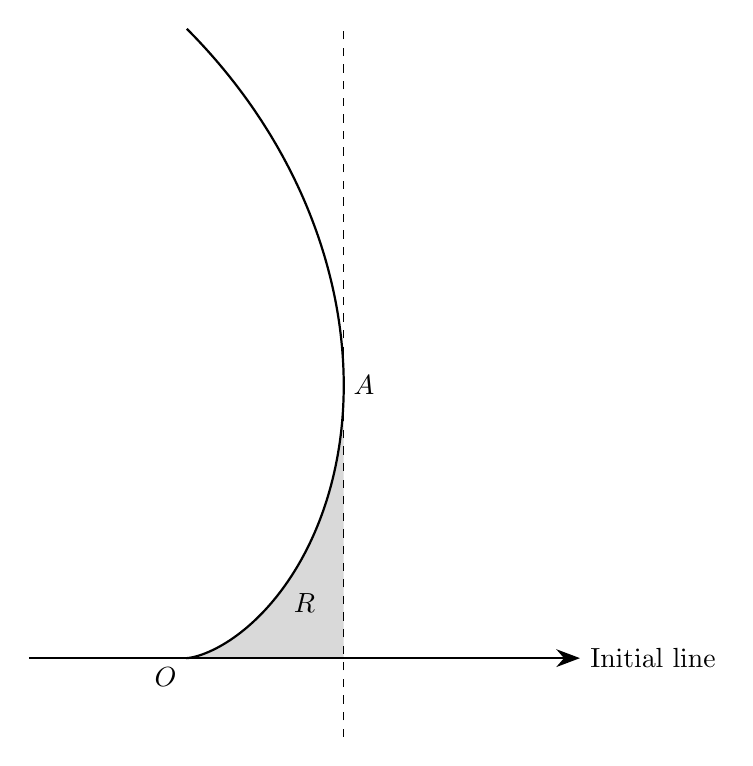
\begin{tikzpicture}[scale=2]
\pgfmathsetmacro{\thA}{pi/3}
\pgfmathsetmacro{\thmax}{pi/2}
\pgfmathsetmacro{\xA}{1}
\pgfmathsetmacro{\yA}{sqrt(3)}

\coordinate (O) at (0,0);
\coordinate (X) at (\xA,0);
\coordinate (A) at (\xA,\yA);
\coordinate (Rlabel) at ($(O)!0.55!(A)+(0.2,-0.6)$);

\fill[gray!30]
  (O)
  plot[smooth, samples=200, domain=0:\thA]
    ({4*(1-cos(deg(\x)))*cos(deg(\x))},{4*(1-cos(deg(\x)))*sin(deg(\x))})
  -- (X)
  -- cycle;

\draw[-{Stealth[length=3mm]}, thick] (-1, 0) -- (2.5,0) node[right] {Initial line};
\draw[dashed] (\xA,-0.5) -- (\xA,4);
\draw[thick]
  plot[smooth, samples=200, domain=0:\thmax]
    ({4*(1-cos(deg(\x)))*cos(deg(\x))},{4*(1-cos(deg(\x)))*sin(deg(\x))});

\node[below left] at (O) {$O$};
\node[right] at (A) {$A$};
\node at (Rlabel) {$R$};
\end{tikzpicture}
\end{figure}


The diagram above shows a sketch of the curve $C$ with equation
\[
r = 4(1 - \cos \theta) \qquad 0 \leq \theta \leq \frac{\pi}{2}
\]
\\
The diagram above also shows the tangent to $C$ at the point $A$, where $A$ is not the pole. \\
This tangent is perpendicular to the initial line. \\

\begin{enumerate}[label=\textbf{(\alph*)}]
  \item Use differentiation to prove that the polar coordinates of $A$ are $\left(2, \dfrac{\pi}{3}\right)$. \marks{4} \\
\end{enumerate}
The finite region $R$, shown shaded in the diagram above, is bounded by $C$, the tangent at $A$ and the initial line. \\
\begin{enumerate}[label=\textbf{(\alph*)}, resume]
  \item Use calculus to show that the exact area of $R$ is $\frac{1}{2}(15\sqrt{3} - 8\pi)$. \marks{6} \\
\end{enumerate}

\newpage

% ---- Question 8 ----
\questionitem

\begin{figure}[H]
    \centering
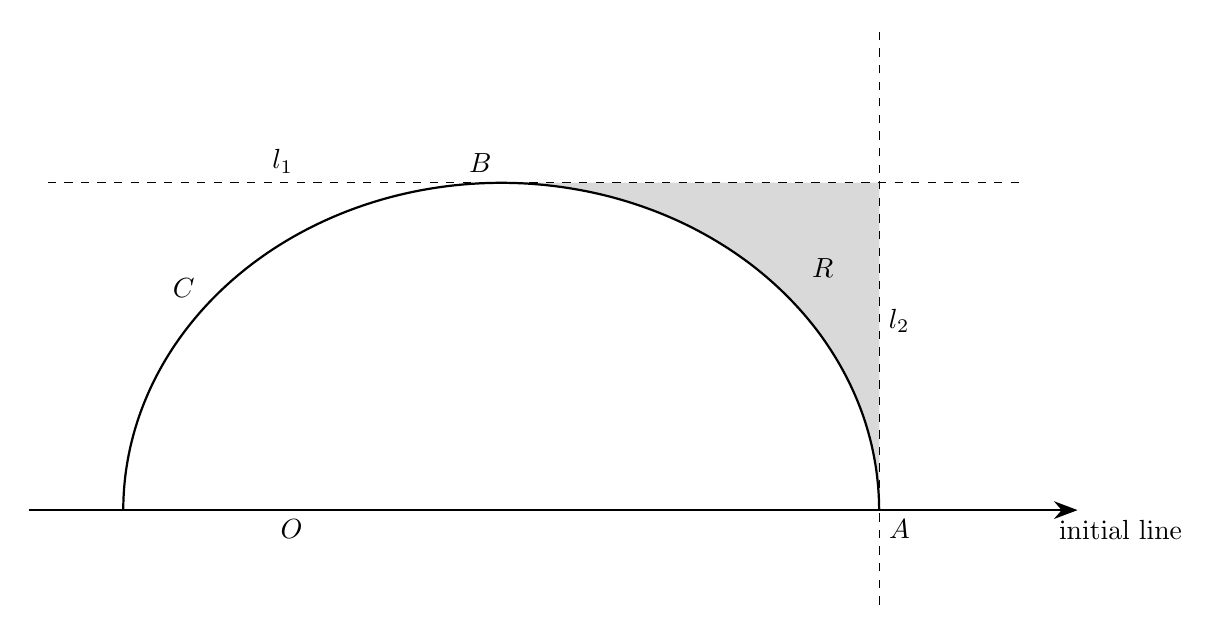
\begin{tikzpicture}[scale=1.2]
\def\a{6}
\def\thB{60}
\pgfmathsetmacro{\xA}{\a}
\pgfmathsetmacro{\rB}{\a/(2-cos(\thB))}
\pgfmathsetmacro{\xB}{\rB*cos(\thB)}
\pgfmathsetmacro{\yB}{\rB*sin(\thB)}
\pgfmathsetmacro{\xC}{\a*cos(118)/(2-cos(118))}
\pgfmathsetmacro{\yC}{\a*sin(118)/(2-cos(118))}

\coordinate (O) at (0,0);
\coordinate (A) at (\xA,0);
\coordinate (B) at (\xB,\yB);
\coordinate (T) at (\xA,\yB);
\coordinate (Rpos) at ($ (B)!0.6!(T) + (1,-0.9) $);

\fill[gray!30] (B) -- (T) -- (A) --
  plot[smooth, samples=120, domain=0:\thB, variable=\t]
    ({\a*cos(\t)/(2-cos(\t))},{\a*sin(\t)/(2-cos(\t))})
  -- cycle;

\draw[dashed] (-2.8,\yB) -- (7.5,\yB);
\draw[dashed] (\xA,-1) -- (\xA,5.1);
\draw[-{Stealth[length=3mm]}, thick] (-3,0) -- (8.1,0);

\draw[thick]
  plot[smooth, samples=200, domain=0:180, variable=\t]
    ({\a*cos(\t)/(2-cos(\t))},{\a*sin(\t)/(2-cos(\t))});

\node[below left] at (O) {$O$};
\node[below right] at (A) {$A$};
\node[above left] at (B) {$B$};
\node[above left] at (\xC,\yC) {$C$};
\node at (Rpos) {$R$};
\node[above left] at (-0.1,\yB) {$l_1$};
\node[right] at (\xA,2.0) {$l_2$};
\node[below right] at (7.8,0) {initial line};
\end{tikzpicture}
\end{figure}


The figure above shows a sketch of the curve $C$ with equation
\[
r = \frac{6}{2 - \cos \theta} \qquad 0 \leq \theta \leq \pi
\]
\\
Given that $C$ meets the initial line at the point $A$, as shown in the figure above \\
\begin{enumerate}[label=\textbf{(\alph*)}]
  \item write down the polar coordinates of $A$. \marks{1} \\
\end{enumerate}
The line $\ell_1$, also shown in the figure above, is the tangent to $C$ at the point $B$ and is parallel to the initial line. \\
\begin{enumerate}[label=\textbf{(\alph*)}, resume]
  \item Use calculus to determine the polar coordinates of $B$. \marks{4} \\
\end{enumerate}
The line $\ell_2$, also shown in the figure above, is the tangent to $C$ at $A$ and is perpendicular to the initial line. \\

The region $R$, shown shaded in the figure above, is bounded by $C$, $\ell_1$ and $\ell_2$. \\
\begin{enumerate}[label=\textbf{(\alph*)}, resume]
  \item By first obtaining a Cartesian equation for $C$, use algebraic integration to find the exact area of $R$, giving your answer in the form $\sqrt{3}(p + q\pi)$ where $p$ and $q$ are constants to be determined. \marks{8} \\
\end{enumerate}


\end{enumerate}
\end{document}
